\chapter{Notes for a Seminar on Anarchist Ideology}
\chapterauthor{Roger A. McCain}

1) Is There any such things as anarchist ideology? Should there be? It is possible to argue that there should not, depending on how we define the term ``ideology". I am defining ideology rather broadly, to refer to any body of interrelated ideas, ideals and hypotheses of fact, which form the basis of discussion and action within a community of interest or purpose. I take it that anarchists are a community of purpose --- we share the purpose of dissolving the political state --- and that we have some ideas in common, and that there is nothing wrong with that.\\
Some ideologies, of course, are founded on the authority of some pope or chairman. Clearly ours cannot be so. The body of ideas which we share is itself, not only the basis for ongoing discussion, but the product of the past discussions and experience of all of us. That is why I title my essay ``Notes for a \emph{Seminar} in Anarchist Ideology." The word ``seminar," I'm told, comes from the Latin for ``manure," the reference being to a field which is well-manured and therefore fertile. In the ivory tower, a seminar is supposed to be a group of scholars, well-manured with knowledge, and thus a fertile field in which new ideas may sprout. I hope my discussion will lead to such an interchange among us more-or-less well-manured anarchists\footnote{Several of these topics are explored at greater length in R.A. McCain, ``Anarchy as a Norm of Social Choice," forthcoming in the \emph{Proceedings of the City College Conference on Social Choice}, edited by Robert Leiter, (Dept. of Economics, City College, CUNY, Convent Ave. at 138th St., New York, New York 10031).}.\\

2) Probably no one will disagree if I say that the central place in the anarchist ideology belongs to the ideal of free agreement. For an anarchist, free agreement is the only legitimate means of resolving conflicts among individuals and groups in society. For example, majority rule is rejected: differences between the majority and the minority ought to be resolved by free agreement, and not by the rule of one group overt the other.\\
Of course, free agreement is a vague term, but it is no vaguer that other popular political terms, including, now that I think of it, ``popular." ``Majority rule," for example, leaves a whole sheaf of questions unanswered: A majority of whom? When? What part would representatives play? How contested? Who makes the agenda, and in what order are the questions taken? What happen when, as is usually the case, there is no majority, but many minority factions? Indeed, the question, ``in what order are the questions taken" appears trivial, but often turns out to be the main reason why one outcome is favored over another\footnote{See Robin Farquharson, \emph{Theory of Voting} (New Haven; Yale University Press, 1969).}.\\
Perhaps we cannot offer a formal definition of ``free agreement" which would be satisfactory. We can, however, agree on some things that free agreement is not. It seems apparent that ``agreements" in which the threat of violence plays some part are not free agreements. This would imply that no free agreement with government is possible, and that the agreements of prisoners cannot be free, since the threat of violence can never be fully excluded in those cases. It would seem also that ``agreements" based on fraud and deceit are not free, even when the deceit is no more that the concealment of relevant information.\\
Even if it does not amount to a formal definition, this is clear enough to be useful. Indeed, some statists would argue that a society based on free agreement is impossible, ``utopian." Clearly that is not so. Kropotkin's \emph{Mutual Aid}\footnote{P. Kropotkin, \emph{Mutual Aid}, has probably been reprinted more often than any other anarchist tract, and several editions are available} and \emph{The Conquest of Bread}\footnote{P. Kropotkin, \emph{The Conquest of Bread}, (Bronx, N.Y.; Blom, 1913, 1968).} showed that most of the useful activity even of the present society is based on free agreement, and that this has been the case throughout history. The importance of force in getting things done is, at best, very much exaggerated.\\

3) Free agreement is a normative, or ethical ideal. Much of the anarchist ideology consists of hypotheses of fact, and the evidence and historical interpretations which support them. Mych of this theory is tacit: that is, the hypotheses are not explicitly stated, but are expressed as criticism of conventional statist ideas, or are implicit in the evidence itself, which is directly cited. There is, I think, some value in stating these hypotheses explicitly, if only for clarity of expression in our discussion with others.\\
One hypothesis which seems to me to be a part of anarchist ideology is the so-called ``iron law of oligarchy."\footnote{The ``iron law of oligarchy" was stated in Robert Michels, \emph{Political Parties}, Tr. Eden and Cedar Paul (New York; Dover, 1959) cited in Mancur Olson, \emph{The Logic of Collective Action}, (New York; Schocken, 1968).} The iron law of oligarchy states that large mass organizations are inevitably run by small intensely involved groups at the top, that is, by oligarchies. Michels, who was the first explicitly to state the law, based it on his study of the German Social-Democratic party. My own knowledge of the historical record suggests to me that this indeed a valid law of sociology. Mancur Olson\footnote{Op. Cit.} has provided a theoretical rationale for the law, based on the assumption that individuals act in accordance with their own purposes (which may or may not be egotistic) within the limits of nature and social arrangements. (That is, his theory is based on the microeconomic concept of utility maximization). Olson's theories go beyond the negative ``iron law" to suggest the remedy: large organizations must not be ``mass organizations" but must be federations of fairly small, local groups. This has, of course, been the anarchist practice.\\
Another possible response to the iron law of oligarchy is to require that all organizations be voluntary. A voluntary organization may be run by an oligarchy, but the oligarchy will find its power limited by possibility that everyone else will leave the organization. Really, the ``iron law of oligarchy" is a problem only in compulsory organizations, such as states; thus it constitutes a strong argument for the abolition of compulsory organizations.\\

4) Federation, voluntary organization, and the preference for small organizations have something to do with free agreement, as well as with the ``iron law," of course. It is perhaps easier to settle differences by free agreement within small groups. Where there are differences between the chapters of a large organization, one way to settle them is for one chapter to secede from the greater organization. A federal form of organization permits this. Small groups, loose federation, and large numbers promote diversity. Within a diversity, the individual is more likely to find a group with which he can willingly affiliate himself, making the resolution of differences withing groups, by means of free agreement, easier. In the case of difference between an individual and his group, the difference must be settled by free agreement again, and on way is the secession of the individual from the group. Where this is not possible, free agreement does not exist. Thus all organizations must be voluntary\footnote{Of course, this discussion owes a great debt to the ideas of the late Paul Goodman, esp. \emph{People of Personnel}, (New York: Vintage Books, 1968). Published with \emph{Like a Conquered Province} by the same author.}. These concepts fit together so intimately that it is no wonder that the ``iron law" has not been separately stated by anarchists.\\

5) Another hypothesis of fact, which anarchists share with new-deal liberals, monarchists, and other advocates of strong discretionary government, is the hypothesis of the incompetence of law. This hypothesis holds that the human reality is too complex and various to be resolved by law. Each case is in principle distinct, so that law must in any case be interpreted. However, a law which must be interpreted is a mere swindle, and in any case, high-minded slogans about ``a government of laws, not of men" are at best obfusc\footnote{I associate the hypothesis of the incompetence of law primarily with Proudhon, and most anarchists take it for granted, but I am not aware of any previous, compact statement of the hypothesis as such.}.\\
The hypothesis of incompetence of law leads the governmentalist back to absolute power, or, at least, to administrative discretion. It also demolishes the pretty constituationalist dream of a society in which differences are resolved by law, democratically arrived at. There are, in fact, only two principles available for the resolution of differences: free agreement and discretionary force. Free agreement recognizes precisely that every case is in principle distinct by dictating nothing in advance, leaving all details \emph{equally} to the parties involved in any dispute.\\

6) We should also observe that free agreement means that agreement is required, not for action but for restraint. This is a parallel between the anarchist ideology and the statist ideology of Hobbes, but it distinguishes anarchism from an important stream of statist thought among economists. This school, or rather group of schools, is often referred to as the ``pubic choice school;" Mancur Olson, whose book was mentioned above, is one member of the school, which has both liberal and conservative branches. Despite the differences of values, the work of this school should be of some interest to anarchists\footnote{The Center for the Study of Public Choice, at Virginia Polytechnic Institute and State University, Blacksburg, Va., is a major clearing house for research results, and they publish the journal \emph{Public Choice}. The Center is associated with a conservative ideology, but not in any official way.}.\\
The basic value premise of the public choice school is the norm of a Pareto Optimum. A Pareto Optimum\footnote{After the Italian economist and sociologist, Vilfredo Pareto. The term is misleading, as there are actually infinitely many possible Pareto optima, corresponding to different allocations between mine and thine.} is an allocation of resources such that no one can be made better off without making someone else worse off, for example by reorganization, shifting resources to alternate uses, introducing known techniques where they are not yet used, etc. Now, on the one hand, that would seem a pretty easy norm to accept: it's an ill wind that blows nobody good, right? On the other hand, it would seem to be an easy standard to live up to: it seems to the casual observer that whenever one person is made better off, another person is almost certain to be made worse off. But that is shortsighted. It is true that ripoffs are as common in this society as fleas on a dog, but that is not to the point. Almost anything constructive can in principle be organized so that nobody is made worse off. It's true that people mostly don't bother, but that's precisely the problem: There has probably never been a society which attained a literal Pareto Optimum.\\
The Public Choice school begins from the premise that such an optimum ought to be attained, or approached as nearly as feasible. In an ideal world free markets and laissez-faire might lead to its attainment, but we do not live in an ideal world, and so some degree of government intervention is supposed to be necessary in order to attain a Pareto Optimum. For conservatives, legal reforms are what is required; for liberals, discretionary government policy. Yet, in principle, even that is not enough. To attain a Pareto Optimum, it would be necessary to have unanimous agreement before any action would be undertaken. Notice that this is precisely the opposite of the anarchist (and the social-contractarian) view of things. Free agreement means that unanimous consent is required for any \emph{restraint} of action. This is an opposite extreme (although a Pareto Optimum, a \emph{distinct} Pareto Optiumum, \emph{might} be attained by a perfect system of free agreement).\\
This can best be illustrated by an example involving the pollution of a common resource, such as air or water. Consider a lake which is shared by a paper plant and a fishing camp. The paper plant dumps its waste in the water, destroying the fish and ruining business for the fishing camp. It can be shown that the profits lost by the fishing camp will always be greater that the profits gained by the paper plant, so that if the two firms were merged, the management would take the profits of the fishing camp into account when deciding what pollution-abatement steps to take, and the owners of both companies could be better off, the gain in profits by the fishing camp being more than enough to compensate the former owners of the paper plant for the cost of pollution abatement. Another way to resolve the problem is to pass a law requiring that before any paper plants are built, the would-be builder must get the permission of the neighbors and buy off any one those who object. This is what I mean when I say that the Public Choice school often seems to require unanimous consent before any action may be taken. This sort of legal regulation is clearly not consistent with free agreement. The merger of the two firms may be, and the third possibility, that the owners of the fishing camp bribe the owners of the paper plant to abate or vacate, is also consistent with free agreement.\\
However, these two resolutions which seem consistent with free agreement are not really solutions, in the long run. The story does not end there. The problem of pollution (according to the economic theory of efficiency) is not pollution \emph{per se} but the fact that pollution is a means of shifting costs onto others, as when the paper manufacturers shift their waste-disposal costs onto others by dumping wastes too cheaply into the lake. The result is that ``too much" paper is made, in this sense: the price of a ream of paper does not include any allowance for the shifted cost of waste disposal. That is, of course, fine from the consumers' point of view, if she gets the profit. However, the price is the money measure of the pleasure and satisfaction of using one ream of paper, or of the satisfaction which would be given up if we should have to give up one ream of paper. The cost of that one ream of paper is greater: it includes not only money costs but also pollution costs. In other words: the ``last" ream of paper produced added more to the cost and sacrifice from making paper that it added to the pleasure and satisfaction of using paper. Thus there ``should" have been at least one less ream of paper made. Just how many less should have been made, we do not know. We do know, though, that if paper-makers can attract bribes, or mergers on terms favorable to them, this fact will attract sharp characters to build paper plants, or to threaten to build paper plants, for the sole purpose of getting bribes or favorable mergers. Thus there will still be ``too much" paper produced, just as there would be if the government subsidized paper making out of the general revenue\footnote{This example is abstracted from a large literature on environmental economics}.\\
In one sense, this is a false problem. The threat to build a polluting plant --- or to fire people from their jobs if depollution standards are raised --- is a threat, and thus may well be inconsistent with the norm of free agreement. I say it may be, because the pollution threat is nonviolent as it was described but 1) some anarchists would exclude even nonviolent threats, 2) if nonviolent threats are admissible, then they are equally admissible for both sides, and the neighbors would be free to counter with nonviolent threats of their own, which might well be sufficient\footnote{See Gene Sharp, \emph{The Politics of Nonviolent Action} (Boston: Porter Sargent, 1973) for a manual of ways and means.}, 3) we might well judge that in reality, pollution is a violent act, which endangers life and health of those subjected to it, and so is to be excluded under free agreement.\\
In any case, it is clear that the false problem brings plenty of real problems along with it. How are we practically to exclude threats? What means of resistance are admissible? How can we, even in principle, tell a ``threat" from a ``promise"?\\
The point of this long digression is that free agreement is a subtle idea, and that economic theory can be useful in exploring it. It is also that the concepts of threat and coercion are equally subtle, and that there is need for more analyses of these subjects from the point of view of economic theory, philosophy, sociology, political ``science," anthropology, psychology and all the rest\footnote{The Institute for Legal and Political Philosophy publishes yearbooks under the title \emph{Nomos}, each organized around a particular subject. A recent volume of \emph{Nomos} was on coercion. I do not have the exact reference at hand, but the symposium in that yearbook is a good instance of the problems with the concept of coercion, and also of the kind of research which needs to be done.}.\\

7) This raises a related question. Some kinds of decisions ought to be made by the public, because they involve everybody in the outcome; that is to say, they are public decisions regardless whether the organizations which make them are public or private. When a despot in a corporate boardroom decides that the Zilch Corporation will not depollute, he is deciding, on behalf of all of us who live near the Zilch Corporation (which \emph{he} generally does not) that the air we breath will be rotten. That decision may be right --- though there are good reasons to doubt it --- but it ought to be a public decision; for a private person to make it on the basis of private calculations is not private enterprise, but despotism.\\
If some decisions must in the nature of things be public decisions, then there must be public organizations to make them. However, an anarchist requires that all organizations be voluntary. Can an organization be both voluntary and public?\\
An approach to this question requires definitions of the terms ``public," and so on, and these are, again, difficult terms. However, Albert Hirschman's fascinating little book, \emph{Exit, Voice and Loyalty}\footnote{(New Haven: Yale University Press, 1971)}, offers some useful insights. How is a person to respond if an organization which provides him with some service, good or utility does not perform satisfactorily? How, for example, is a person to respond if the telephone service he receives is unsatisfactory? He can raise bell about it; this is a resort to \emph{voice}. Alternatively, he can stop doing business with those cruds, and this is a resort to \emph{exit}. Organizations differ both in their responsiveness to exit and to voice and in the cost of exit and of voice. For example, the telephone company would probably be rather responsive to exit: as a more or less private firm they would find the loss of revenues from large-scale exit ruinous. However, the cost of exit is very high, since a person who refuses to do business with the phone company will have to do without a telephone, and there are no close substitutes. If there were two or more telephone companies within an area, or other services available which would be a close substitute, then the cost of exit from the telephone company would be much lower. Governments, by claiming territorial jurisdiction over large areas, make the cost of exit quite high. It is sometimes said that people have no right to complain about the conditions in the United States, since they are free to leave. But ``free?" The cost of exit is enormous: one must leave one's home, one's friends, one's language, a very large portion of one's life, not to mention the world's third-highest standard of living. On the other hand, repressive states so to some trouble to make the cost of voice high, while democratic states are supposed to be highly responsive to voice, especially the ceremonially proper resort to voice we call ``voting."\\
Consideration of the cost of exit raises the related issue of the cost of entrance. If the cost of entrance is high, then 1) people will be less likely to exit, since they will not wish to forfeit their initiation fees; 2) they will be less likely to be discontented in the first place, because discontent will cause cognitive dissonance; 3) if other organizations which provide substitute services have high costs of entry, then the effect is the same as if the organization one currently patronizes has a high cost of exit. Communist parties, religious orders and industrial oligopolies have high costs of entrance. The cost of entering a hereditary aristocracy is essentially infinite.\\
I would define a \emph{public} organization as one which has a low cost of entry, or none, and which is highly responsive to voice. Notice that this would include ideal democratic governments but also includes food conspiracies\footnote{It includes food conspiracies in principle. In fact --- I know of at least one food conspiracy in which the rhetoric about everyone being welcome is self-deception, and in fact only a small in-group is allowed to participate. There are no rules forbidding nongroup participants, but there is no formal organization either, and unless you know the ingroup very well, you just cannot find anybody who will cooperate with you. I do not condemn the group for that, but only for lying to themselves about what it is they are doing. Cost of entrance does exist in fact, and it is igh. It is not enough that there are no formal rules specifying a high cost of entry: the absence of positive action to facilitate entry is often enough.}, most chess clubs, Kibbutzim, industrial labor unions, and many other nongovernmental organizations. I would define a \emph{voluntray} organization as one with a low cost of exit, or none. This would include competitive business firms (from the consumer's point of view, that is) anarchist federations, most chess clubs, craft labor unions, the Playboy subscriber list, and the Pepsi Generation. There is no reason why organizations cannot be both public and voluntary on this view; most chess clubs are.\\
I do not mean to suggest that all organizations in an anarchist society must be both public and voluntary. Nonpublic organizations have their uses: it is clearly appropriate for a cooperative mutual-aid society to require that its members contribute something to the common fund as a condition of membership. What I do mean is to say that anarchists are not obliged to oppose all \emph{public} organizations, simply because it is public, and that an anarchist federation should be a public organizations, or indeed if he offers arguments that on the contrary it should not. I do mean that we can demand that labor organizations be voluntary and public, without uttering nonsense. I do mean that we may demand, without self-contradiction, that banking and finance be carried on by public organizations in an anarchist society, and in general to talk about public organization in an anarchist society and about the Anarchist Republic (Res Publica, ``public thing.")\\

\begin{figure}[t]
\begin{center}
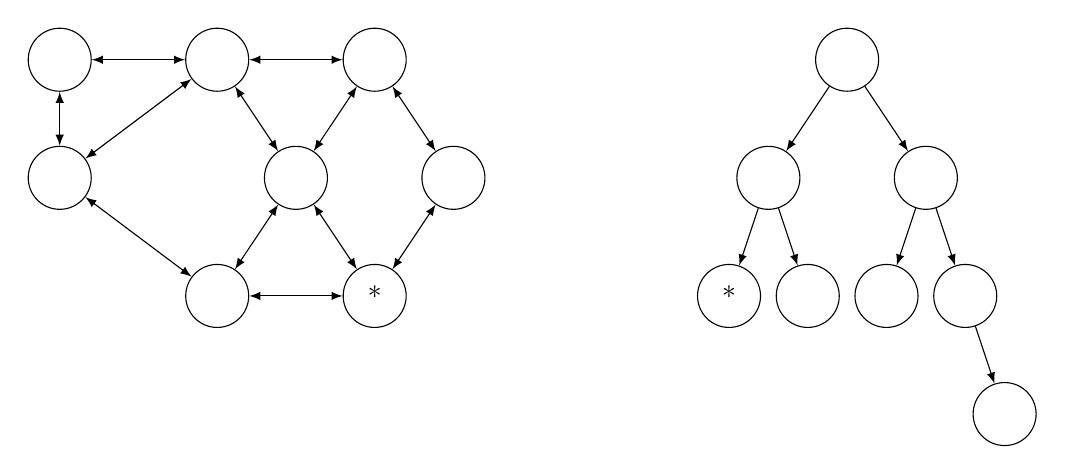
\begin{tikzpicture}
	%Network
	\node[draw, circle, minimum size=0.8cm] (0) at (0,0) {};
	\node[draw, circle, minimum size=0.8cm] (1) at (2,0) {};
	\node[draw, circle, minimum size=0.8cm] (2) at (4,0) {};
	\node[draw, circle, minimum size=0.8cm] (3) at (0,-1.5) {};
	\node[draw, circle, minimum size=0.8cm] (4) at (3,-1.5) {};
	\node[draw, circle, minimum size=0.8cm] (5) at (5,-1.5) {};
	\node[draw, circle, minimum size=0.8cm] (6) at (2,-3) {};
	\node[draw, circle, minimum size=0.8cm] (7) at (4,-3) {*};
	\draw[<->, >=latex] (0) -- (1);
	\draw[<->, >=latex] (0) -- (3);
	\draw[<->, >=latex] (1) -- (2);
	\draw[<->, >=latex] (1) -- (3);
	\draw[<->, >=latex] (1) -- (4);
	\draw[<->, >=latex] (2) -- (4);
	\draw[<->, >=latex] (2) -- (5);
	\draw[<->, >=latex] (3) -- (6);
	\draw[<->, >=latex] (4) -- (6);
	\draw[<->, >=latex] (4) -- (7);
	\draw[<->, >=latex] (5) -- (7);
	\draw[<->, >=latex] (6) -- (7);
	
	%Hierarchy
	\node[draw, circle, minimum size=0.8cm] (10) at (10,0) {};
	\node[draw, circle, minimum size=0.8cm] (11) at (9,-1.5) {};
	\node[draw, circle, minimum size=0.8cm] (12) at (11,-1.5) {};
	\node[draw, circle, minimum size=0.8cm] (13) at (8.5,-3) {*};
	\node[draw, circle, minimum size=0.8cm] (14) at (9.5,-3) {};
	\node[draw, circle, minimum size=0.8cm] (15) at (10.5,-3) {};
	\node[draw, circle, minimum size=0.8cm] (16) at (11.5,-3) {};
	\node[draw, circle, minimum size=0.8cm] (17) at (12,-4.5) {};
	\draw[->, >=latex] (10) -- (11);
	\draw[->, >=latex] (10) -- (12);
	\draw[->, >=latex] (11) -- (13);
	\draw[->, >=latex] (11) -- (14);
	\draw[->, >=latex] (12) -- (15);
	\draw[->, >=latex] (12) -- (16);
	\draw[->, >=latex] (16) -- (17);
\end{tikzpicture}
\caption{\label{Fig1}}
\end{center}
\end{figure}
8) Yet another way of saying the same thing is to say that anarchists are opposed to hierarchies. Because a hierarchy implies the resolution of differences by submission of one to another, it seems that hierarchy is inconsistent as a principle with free agreement. We might be willing to go along with hierarchical structures of voluntary organizations. That is a debatable point in principle, but in practice hierarchical organizations impose high costs of exit, that is, they are not in practice voluntary as a rule.\\
Structure is a necessity, to be sure, but anarchists urge the virtues of networks rather than hierarchies. (By the way, the so-called broadcast networks are actually hierarchies. That is what is wrong with them). Examples of the two forms are contrasted in the simple-minded diagram in Figure \ref{Fig1}. There are two important differences. In a network, the flow of information and influence is two-way, while in a hierarchy the flow of influence is downward ans the flow of information is either upward or downward but only ``through channels." It would appear that the hierarchy is a way to speed communication but (quite apart from the complications of communication between unequals) this is not so. Communication from the representative member of the group marked with an asterisk in the network to another arbitrarily chosen number will require an average of 1.86 connections or passages from one person to another. The comparable number for the asterisk-marked member in the hierarchy is exactly three. There are, of course, more lines of communication in the network -- eleven versus seven -- and interestingly enough, the product of the number of successive messages required times the number of channels required to keep the members in contact is about the same: 20.86 for the network, 21 for the hierarchy. This suggests to me that the two are about equally ``efficient" in some as yet undefined sense.\\
There is an old saying that human groups cannot be gotten together very easily, because whenever two groups join together one must be subjected to the other, and neither group will accept that willingly. This is true, so long, and only so long, as they are both organized in hierarchies. Figure \ref{Fig2} illustrates the point. The two hierarchies cannot be joined together without subjecting the boss of one or the other or both of them, as the one marked by the asterisk would be subordinated to the leader of the other group. It is not the rank-and-file who must be subordinated in order to join the two groups together, but the man who will make the decision whether to joint or not --- and he, of course, will resist subordination to the other hierarchy. Networks, however join readily and in a natural way, as illustrated in Figure \ref{Fig3}. Joining the two networks requires, at a minimum, only a link such as that between the two members marked with asterisks. This does not change the fundamental role of either of the members forming the link, though it increases their work load somewhat (this does not change the fundamental role of either of the members forming the link, though it increases their work load somewhat (this could be compensated by dropping one link, such as the links to the members marked with a \#) and it does not change the nature of either network. The ``law of nature" cited by Galbraith\footnote{Reference is to \emph{The New Industrial State}. Several editions are available.} and others, that ``orgranizations" always defend their autonomy, turns out to be oversimplified and misleading. True of course that the top men in hierarchies always protect their autonomy: others in hierarchies do no have any to protect. True, also, that hierarchies will not cooperate well, for that reason\footnote{Benjamin Ward, \emph{The Socialist Economy}, (New York; Random House, 1967) expands on this point. See ch.5.}. However, and without any sacrifice in the autonomy of either.\\
\begin{figure}[t]
\begin{center}
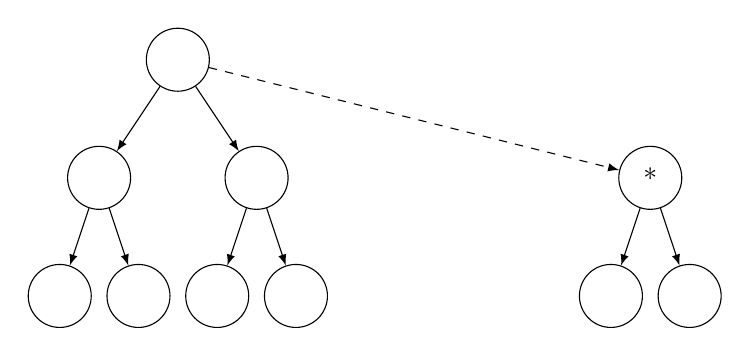
\begin{tikzpicture}
	\node[draw, circle, minimum size=0.8cm] (10) at (10,0) {};
	\node[draw, circle, minimum size=0.8cm] (11) at (9,-1.5) {};
	\node[draw, circle, minimum size=0.8cm] (12) at (11,-1.5) {};
	\node[draw, circle, minimum size=0.8cm] (13) at (8.5,-3) {};
	\node[draw, circle, minimum size=0.8cm] (14) at (9.5,-3) {};
	\node[draw, circle, minimum size=0.8cm] (15) at (10.5,-3) {};
	\node[draw, circle, minimum size=0.8cm] (16) at (11.5,-3) {};
	\draw[->, >=latex] (10) -- (11);
	\draw[->, >=latex] (10) -- (12);
	\draw[->, >=latex] (11) -- (13);
	\draw[->, >=latex] (11) -- (14);
	\draw[->, >=latex] (12) -- (15);
	\draw[->, >=latex] (12) -- (16);
	
	\node[draw, circle, minimum size=0.8cm] (20) at (16,-1.5) {*};
	\node[draw, circle, minimum size=0.8cm] (21) at (15.5,-3) {};
	\node[draw, circle, minimum size=0.8cm] (22) at (16.5,-3) {};
	\draw[->, >=latex] (20) -- (21);
	\draw[->, >=latex] (20) -- (22);
	
	\draw[->, >=latex, dashed] (10) -- (20);
	\end{tikzpicture}
\caption{\label{Fig2}}
\end{center}
\end{figure}

\begin{figure}[t]
\begin{center}
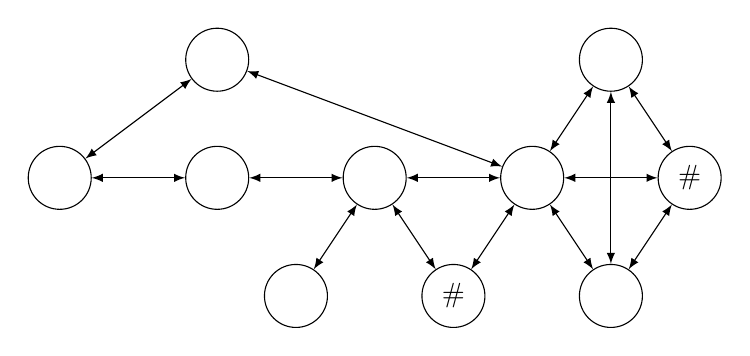
\begin{tikzpicture}
	\node[draw, circle, minimum size=0.8cm] (0) at (2,0) {};
	\node[draw, circle, minimum size=0.8cm] (1) at (7,0) {};
	\node[draw, circle, minimum size=0.8cm] (2) at (0,-1.5) {};
	\node[draw, circle, minimum size=0.8cm] (3) at (2,-1.5) {};
	\node[draw, circle, minimum size=0.8cm] (4) at (4,-1.5) {};
	\node[draw, circle, minimum size=0.8cm] (5) at (6,-1.5) {};
	\node[draw, circle, minimum size=0.8cm] (6) at (8,-1.5) {\#};
	\node[draw, circle, minimum size=0.8cm] (7) at (3,-3) {};
	\node[draw, circle, minimum size=0.8cm] (8) at (5,-3) {\#};
	\node[draw, circle, minimum size=0.8cm] (9) at (7,-3) {};
	\draw[<->, >=latex] (0) -- (2);
	\draw[<->, >=latex] (0) -- (5);
	\draw[<->, >=latex] (1) -- (5);
	\draw[<->, >=latex] (1) -- (6);
	\draw[<->, >=latex] (1) -- (9);
	\draw[<->, >=latex] (2) -- (3);
	\draw[<->, >=latex] (3) -- (4);
	\draw[<->, >=latex] (4) -- (5);
	\draw[<->, >=latex] (4) -- (7);
	\draw[<->, >=latex] (4) -- (8);
	\draw[<->, >=latex] (5) -- (6);
	\draw[<->, >=latex] (5) -- (8);
	\draw[<->, >=latex] (5) -- (9);
	\draw[<->, >=latex] (6) -- (9);
\end{tikzpicture}
\end{center}
\caption{\label{Fig3}}
\end{figure}

9) Fredrick C. Thayer's book, \emph{An End to Hierarchy! An End to Competition!}\footnote{(New York: Franklin Watts, 1973)} sounds like it might be an anarchist-communist tract. It isn't, and indeed the author's commitment to such authoritarian constructs as the MacDonald's hamburger chain, the U.S. Constitution and the National Security Council lend a surrealistic tone to the book's devotion to sweet consensus. Yet the book provides ample evidence of the productivity and importance of small groups, even within such organizations as those, and of the fact taht network structure is indispensable to every organization, however committed to formal hierarchy. Thayer's book is in the tradition of soft-headed or ``theory Y" management studies, as opposed to the hard-headed" or ``theory X" headbusters. However, Thayer's attitude to unions is pure paternalism.\\
Thayer finds that the ideal group size, in management studies, is five. One wonders if he might be a hidden Illuminatus\footnote{Reference is to \emph{Illuminatus!}, by R. Shea and R.A. Wilson, (New York, Dell, 1975) No flattery to the editor of this journal is intended by the mention, of course. Of course.}. A nice exercise for the brain is to read Thayer's book along with Robert Heinlein's \emph{The Moon is a Harsh Mistress}\footnote{(New York: Berkeley, 1968)}, if you can sneer at the militarism the two men share. But this leads us into science fiction, which is a horse of a different feather.\\

10) I think I have said enough, in this laundry list, to make my point. There is such a thing as anarchist ideology, even if it is mostly tacit in things we all take for granted. It is useful in that it helps us to communicate with others. That is a two-way street, and it is pretty certain that some of us don't want to communicate (we just want those others to listen) but it doesn't work that way. We can learn from social science, and even from business management, accounting and finance, if we approach those literatures critically. They can learn from us, maybe, but not unless we learn to communicate our ideas to them, in words, plain words, words that they are accustomed to using. For that we need explicit discussions of anarchist ideology, so that we can first understand one another.\\